\documentclass[12pt]{article}
\usepackage{fancyhdr}
\usepackage{datetime}
\usepackage{enumitem}
\usepackage{amsmath}
\usepackage{graphicx}
\graphicspath{ {images/} }
%\usepackage{showframe}

%custom variables
\newdate{date}{23}{09}{2016}
\newcommand{\hwNum}{1}
\newcommand{\hwTitle}{EC441: Lab 1}


%header
\pagestyle{fancy}
\lhead{Daniel Andronov}
\chead{\thepage}
\rhead{\hwTitle}
\cfoot{\thepage}

\fancyheadoffset[LO,RE]{1pt}
\fancyheadoffset[RO,LE]{1pt}

%titlepage
\title{\hwTitle}
\author{Daniel Andronov}
\date{\displaydate{date}}

%addition settings
\topmargin=-0.45in
\evensidemargin=0in
\oddsidemargin=0in
\textwidth=6.5in
\textheight=9.0in
\headsep=0.25in

\begin{document}
\maketitle
\newpage


\section{Introduction to Traceroute}
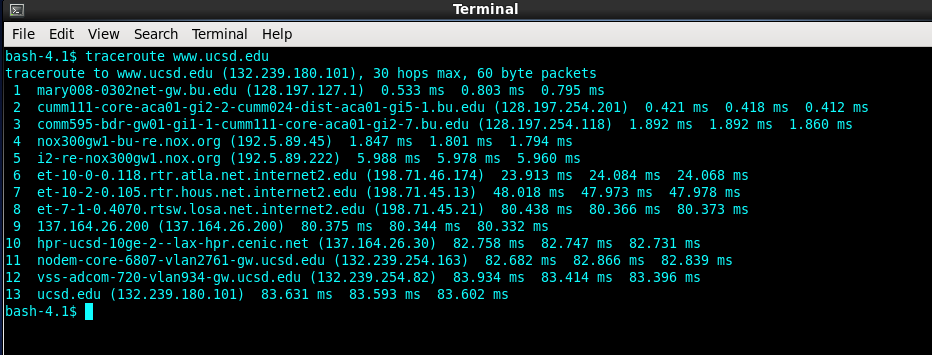
\includegraphics[ width=\textwidth, scale = 0.25 ]{traceroute_0947}

\paragraph{Question 1\\}
\textbf{Solution: }
13 Hops.

\paragraph{Question 2\\}
\textbf{Solution: }
The traceroute seems to indicate that the packet traved through the "altas" and "cenic.net" ISP's. 

\paragraph{Question 3\\}
\textbf{Solution: }
The locations of the routers involved in the traceroute are described in the following table
\begin{center}
	\begin{tabular}{ | l | l | l | l | }
	\hline
	Hop No. & IP address & ISP & Location \\ \hline
	1  & 128.197.127.1 	& Boston University		& Boston, MA \\ \hline
	2   & 128.197.254.201 	& Boston University		& Boston, MA \\ \hline
	3   & 128.197.254.118 	& Boston University 	& Boston, MA \\ \hline
	4   & 192.5.89.45		& Harvard University 	& Cambridge, MA \\ \hline
	5   & 192.5.89.222 		& Harvard University	& Cambridge, MA \\ \hline
	6   & 198.71.46.174	& Internet2			& Ann Arbor, Michigan \\ \hline
	7   & 198.71.45.13.		& Internet2			& Ann Arbor, Michigan \\ \hline
	8   & 198.71.45.21		& Internet2			& Ann Arbor, Michigan \\ \hline
	9   & 137.164.26.200	& CENIC			& Cypress, California \\ \hline
	10 & 137.164.26.30	& CENIC			& Cypress, California \\ \hline
	11 & 132.239.254.163	& UCSD			& La Jolla, California \\ \hline
	12 & 132.239.254.82	& UCSD			& La Jolla, California \\ \hline
	13 & 132.239.180.101	& UCSD			& La Jolla, California \\ \hline
	\end{tabular}
\end{center}

\paragraph{Question 4\\}
\textbf{Solution: }
traceroute www.ucsd.ed -N 10

\paragraph{Question 5\\}
\textbf{Solution: }
The round trip time to the destination was occasionally faster that the intermediate. This is most probably due to some traffic on the route to the destination or that the packet took some longer route that is not shown in the traceroute output. 

\paragraph{Question 6\\}
\textbf{Solution: }

\begin{center}
	\begin{tabular}{ | l | l | l | l |  }
	\hline
	Trial No. & Probe 1 RRT & Probe 2 RRT & Probe 3 RRT  \\ \hline
	1 & 83.526 & 83.511 & 83.423 \\ \hline
	2 & 83.631 & 83.593 & 83.602 \\ \hline
	3 & 85.565 & 83.596 & 84.265 \\ \hline
	4 & 83.494 & 83.391 & 83.906 \\ \hline
	
	\end{tabular}
\end{center}

The RTT to the destiniation has average 83.792 ms and standard devation 0.581 ms.


\section{Wireshark Experiments}

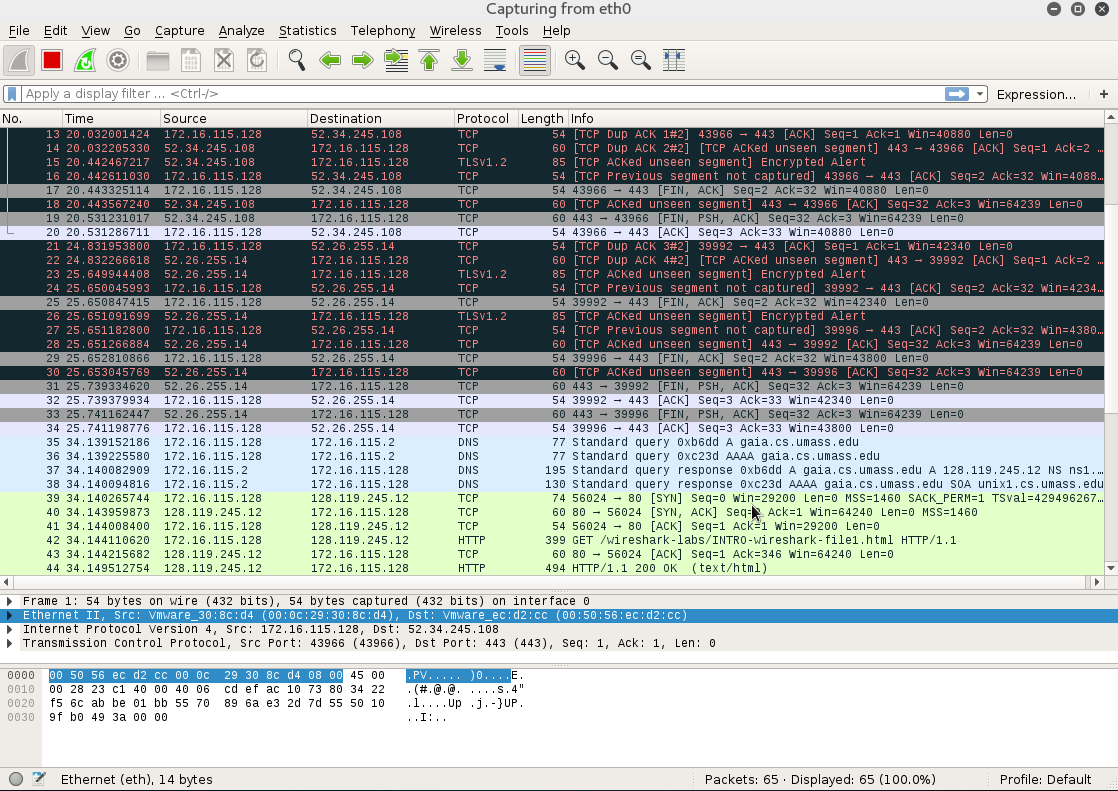
\includegraphics[ width=\textwidth, scale = 0.25 ]{wireshark}
\paragraph{Question 7\\}
\textbf{Solution: }
TCP, HTTP TLSv1.2

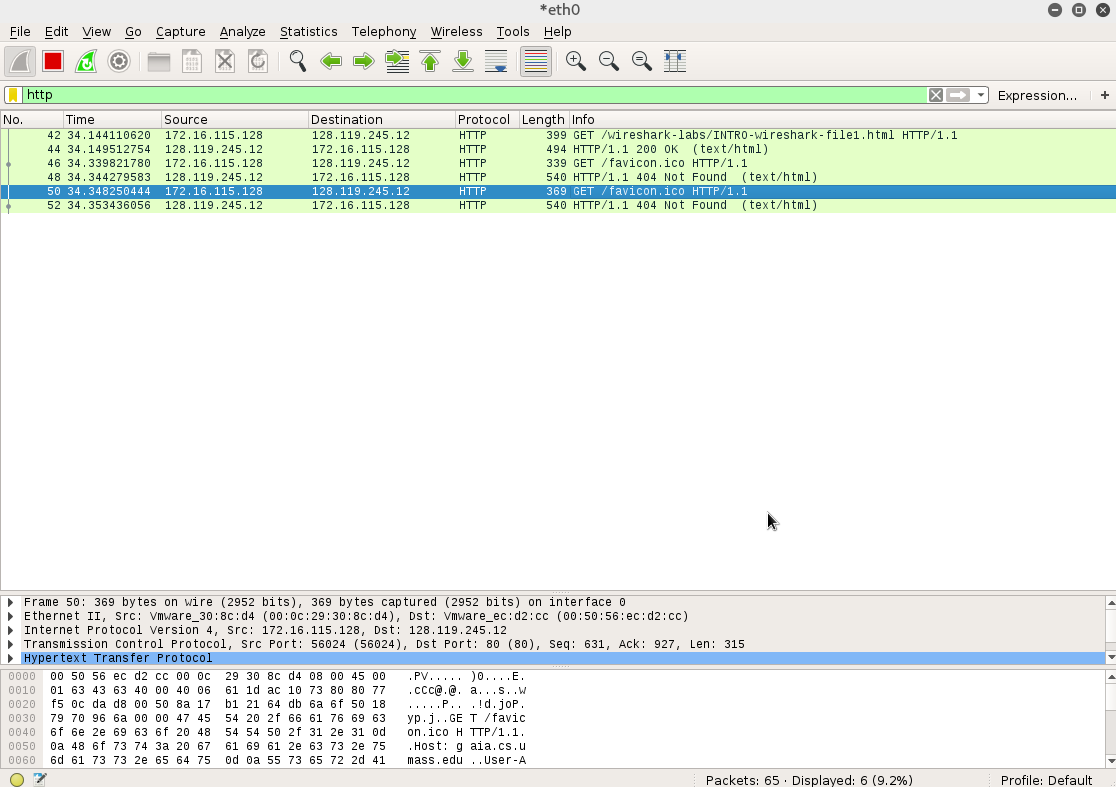
\includegraphics[ width=\textwidth, scale = 0.25 ]{wireshark_http}

\paragraph{Question 8}
\textbf{Solution: }
The GET packet was timestamped at 34.144110620 and the OK packet was timestamped at 34.149512754 sec, so the time in between the two packets was 0.005402134 sec or about 5.4 ms.

\paragraph{Question 9\\}
\textbf{Solution: }
128.119.245.12

\paragraph{Question 10\\}
\textbf{Solution: }
172.16.115.128

\paragraph{Question 11\\}
\textbf{Solution: }
The IP addresses starting with 192.168.x.x and 172.16.x.x are two of three sets of IP adresses reserved for private netorks, with the last reserved address is 10.x.x.x. These three addresses ranges are called classes, with each having more addresses to support connected devices than the last. They are ordered as below. 
\begin{center}
	\begin{tabular}{ | l | l | l |}
	\hline
	Address Range & Class Type & Maximum Devices \\ \hline
	192.168.x.x & A & 65,536 \\ \hline
	172.16.x.x - 172.31.x.x & B & 1,048,576 \\ \hline
	10.x.x.x & C & 16,777,216 \\ \hline
	\end{tabular}
\end{center}


\end{document}
This is never printed